\documentclass{beamer}
\mode<presentation>
{
  \usetheme{Singapore}
  \usecolortheme{wolverine}
%  \setbeamercovered{transparent}
  \setbeamercovered{invisible}
 }
\usepackage[english]{babel}
\usepackage[latin1]{inputenc}
\usepackage{graphicx}
\usepackage{times}
\usepackage[T1]{fontenc}
\usepackage{mathrsfs}
\usepackage{listings}
\usepackage{verbatim}
\usepackage{color, colortbl}
\usepackage{soul}
 \usepackage{tkz-graph}  
% \usetikzlibrary{positioning} 
\usetikzlibrary{shapes.geometric}%   
\newcommand\SoulColor{%
	\let\set@color\beamerorig@set@color
	\let\reset@color\beamerorig@reset@color}
\newcommand*{\Scale}[2][4]{\scalebox{#1}{$#2$}}%

\lstset{
	numberstyle=\footnotesize,
	basicstyle=\ttfamily\tiny}
\graphicspath{{/Graphics}}

%%%%%%%%%%%%%%%%%%%%%%%%%%%%%%%%%%%%%%%%%%%%%%%%%%%%%%%%%%%%%%%5
\title[TND] % (optional, use only with long paper titles)
{Confounding of Influenza VE Estimates by History of Vaccination}
%\subtitle
%{An attempt to vindicate the 'Bayesian approach'}
\author{Ivo M. Foppa}
\date % (optional, should be abbreviation of conference name)
{5/5/2017}
% If you wish to uncover everything in a step-wise fashion, uncomment
% the following command:
%\beamerdefaultoverlayspecification{<+->}
\begin{document}
\begin{frame}
  \titlepage
\end{frame}
\section{Background}
%
\begin{frame}
	
	{\small Ohmit et al. (2014). Influenza vaccine effectiveness in the 2011-2012 season: protection against each circulating virus and the effect of prior vaccination on estimates. \emph{Clinical Infectious Diseases}, 58(3), 319-327.}
	\begin{figure}
		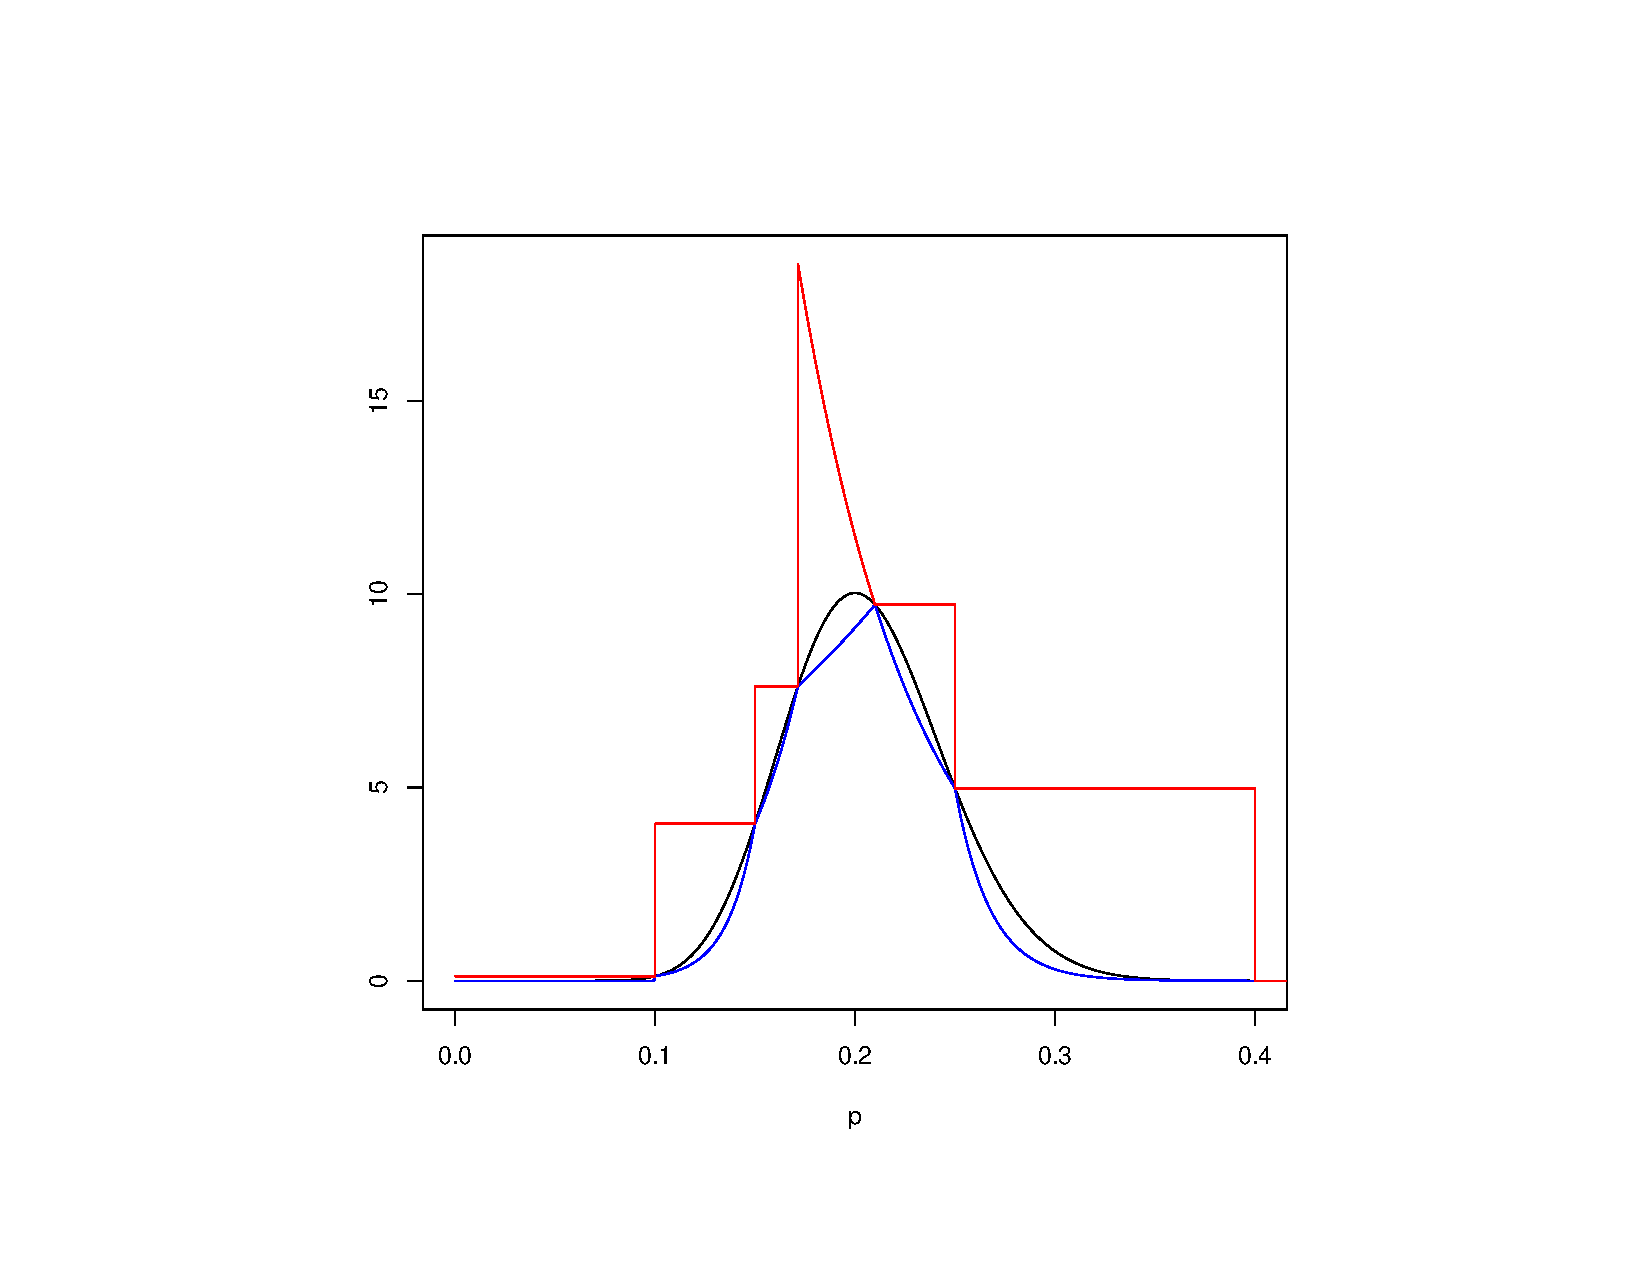
\includegraphics[width = \linewidth]{adaptation_sr1.pdf}
	\end{figure}
\end{frame}
%
%	
\end{document}
